% Chapter 2
\chapter{State of the Art (Literature Review)} % Main chapter title
\label{Chapter2} % For referencing the chapter elsewhere, use \ref{Chapter2} 
\minitoc
%----------------------------------------------------------------------------------------

%% Define some commands to keep the formatting separated from the content 
%\newcommand{\keyword}[1]{\textbf{#1}}
%\newcommand{\tabhead}[1]{\textbf{#1}}
%\newcommand{\code}[1]{\texttt{#1}}
%\newcommand{\file}[1]{\texttt{\bfseries#1}}
%\newcommand{\option}[1]{\texttt{\itshape#1}}

%----------------------------------------------------------------------------------------

This chapter reviews several topics that are relevant for this work. The first section reviews the presence of occupants in a building since it is an important concept to keep in mind during the analysis of time series of the multivariate building dataset. This concept allows the researcher to be aware of the interaction between human beings and a building. The following sections review all the necessary concepts that are used in our proposed methodology.


\section{Important definitions}

Some important definitions that are used in this master thesis:

\begin{itemize}
\item \textbf{Behavior of the builiding} this term expresses the idea that the indoor environment of a building changes depending on external conditions, the interaction with human beings, maintenance operations, or any other phenomena that produces this change.

\item \textbf{Daily profile} is a vector of 24 values that describe the fluctuation of a variable during the day, each value for each hour.

\item \textbf{Cluster daily profile} is a group of days that have similar daily profile for the studied variable. The cluster profile is defined by a mean vector $P_x = \{ \mu_{x_i} \forall i \in [0,23] \}$ and a standard deviation vector $STD_x = \{ \sigma_{x_i} \forall i \in [0,23] \}$ of length $N=24$.
\item  \textbf{Motif cluster profile} is a collection of days that have a typical/common daily profile. This cluster profile appears often in the time series data.
\item  \textbf{Discord cluster profile} is a collection of days that have non-typical/ abnormal daily profiles.

\item \textbf{Label data frame} is a big table that summarizes all the generated labels for each proposed model. It create a mapping between the discovered patterns and a code of identification. 
 
\end{itemize}
 

\section{Occupant presence}

Occupant presence (OcP) in buildings has been investigated for decades. In \citeyear{artf_light_1980}, \citet{artf_light_1980} proposed a method for predicting the use of artificial lighting based on the switching behavior of occupants. His approach uses a logistic curve as a probability density function (\textit{pdf}) for deciding the likelihood of whether a switching activity will occur during the course of a day, according to the occupant presence.
In \citeyear{page_2008}, \citeauthor{page_2008} et al. \citep{page_2008} summarized similar approaches for heating, cooling and ventilation systems, and they proposed a generalized stochastic model for simulation of occupant presence. \citeauthor{page_2008} et al. \citep{page_2008} presented a scheme (figure \ref{fig:OCC_MODEL}) where it is possible to see the means of interaction between occupants and buildings. They claimed that occupant presence is an input to all other models (i.e. water, electrical appliances, lighting utilities, etc.) and the OcP model will be central to the family of other stochastic models.

\begin{figure}[h!]
  \vspace{0.5em} %better style
  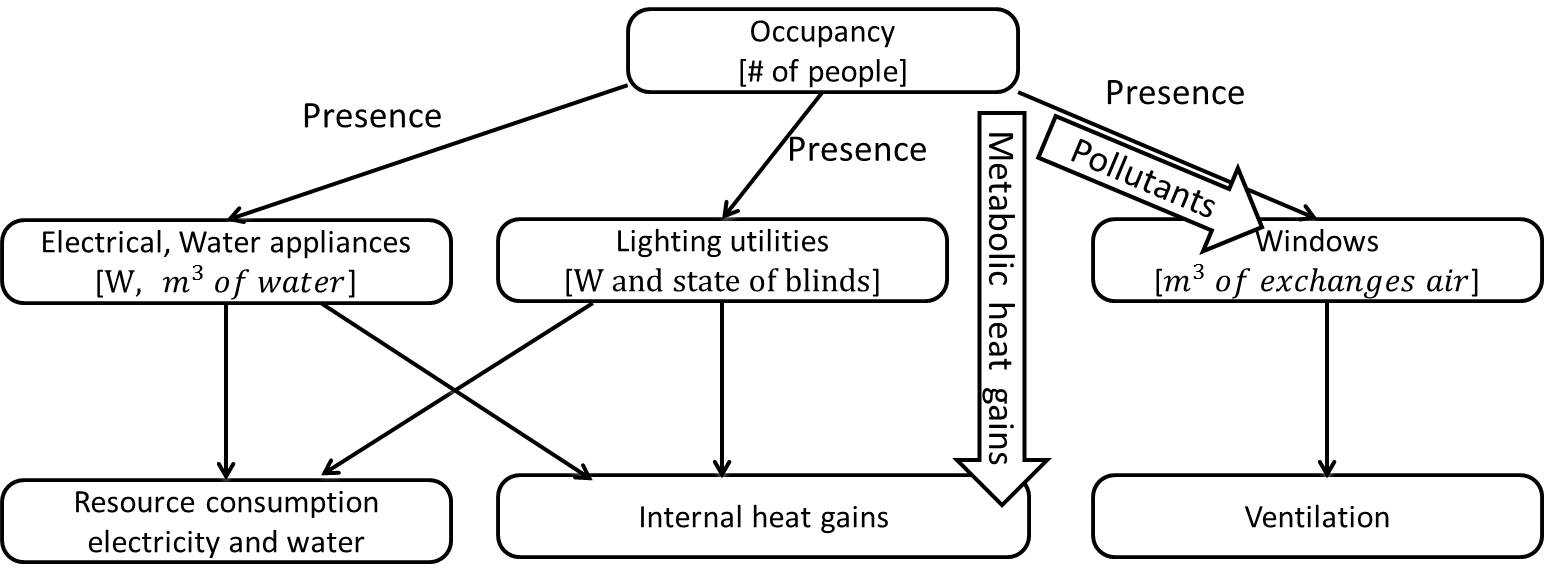
\includegraphics[width=\linewidth]{Figures/Page_presence_scheme.jpg}
  \caption{Outputs of the occupancy model and their later use by stochastic models of occupants’ behaviour. \cite{page_2008}}
  \label{fig:OCC_MODEL}
\end{figure}

Most of the OcP models that are summarized in \citeauthor{page_2008}'s work fit their parameters according to the related presence data. This process, called “calibration process”, was often made by hand or deduced by heuristic techniques. In most cases, the evaluation methods for these models was the measurement of their capacity to reproduce, realistic behavior of the occupants after the calibration process. Having a realistic simulation of occupant presence
is one of the most important aspects for the OcP models, this is because, a lack of an accurate estimation of occupant presence will imply a miscalculation of resources such as water, electric energy and others. Thus, the over- or underestimation of presence is undesirable in the majority of the cases \cite{page_2008, wang_2005, profile_comp_2001}.\\


\citeauthor{wang_2005}, \citeyear{wang_2005} \cite{wang_2005} put into evidence one example of OcP overestimation. In their simulation, they observed peaks of presence in the first hour of the day (which implies overestimation of presence) due to their assumption of the normal distribution of the arrival time in the morning. \citeauthor{wang_2005} were aware of the absent periods of the occupants, and they found that the absence intervals were exponentially distributed and that the coefficient of the exponential distribution for a single office was treated as a constant over the day. To overcome the overestimation problem of presence,  the authors mention the use of empirical distributions for daily events like the arrival in the morning.    


\subsection{Occupancy diversity factors}

Nowadays, one of most the common ways to estimate occupant presence is by using the diversity profiles approach (also called occupancy schedules or occupancy profiles) \cite{profile_comp_2001,davis2010occupancy,duarte2013revealing}(2001, 2010, 2013). This approach consists of daily profiles that are composed of 24-hour representative values. These representative values are a more realistic interpretation of occupant presence because a daily profile does not make assumptions about the probability distribution of daily events such as arrival times in the morning (as it was described before in the example of \cite{wang_2005}). However, this approach could miscalculate the presence of occupants throughout the year when there is a repetition of a subset of profiles that do not consider the temporal variations such as seasonal habits, irregular days (late arrivals or early departures), differences in behavior between weekdays and weekends, and atypical behavior like the presence of people
in office buildings on a weekend \cite{davis2010occupancy}.   \\

To have a more realistic representation of occupant presence, the OcP models would like to be the closest possible to the real behavior of the occupants. However, for simplicity, it is common that the diversity factor for each workday (i.e. usually from Monday to Friday) is treated identically, and weekends treated with a different profile. A typical profile is lower during the absence of the occupants and increases its value during the expected occupancy periods. A maximum factor value is achieved when the maximum expected presence of occupants occurs, or in the case of some types of  HVAC equipment, when weather is over extreme design condition. Duarte et al. 2013 \cite{duarte2013revealing}.  \\

Davis et al. \cite{davis2010occupancy} show examples of OcP profiles of different kinds of buildings. In their work, we can find remarkable differences between workdays for each building type. One example is the library building, where we can see a highest occupancy level on Mondays and a lowest occupancy level on Fridays. For this building, the authors suggested an individual OcP modeling for the following three groups: Monday through Thursday, Friday, and weekend schedules. These groups have what will be called in this work as behavioral coincidence. \footnote{Note that this term will be used in this work. This term indicates a similarity between two or more OcP profiles}      


\subsection{Deterministic and stochastic occupancy factors}
       
\citeauthor{duarte2013revealing} \cite{duarte2013revealing} mention the idea of deterministic and stochastic occupancy factors. According to their criteria, while a deterministic OcP model identifies or creates a standard workday profile which is the same for the whole workweek, a different weekend profile is created for Saturday and Sunday. The deterministic model assumes no change in occupancy schedules throughout the year. On the other hand, a stochastic model uses various probabilistic methods to capture the random nature of individuals’ behavior. Both OcP models are valid for estimating occupancy presence, the former is simple but overestimates occupancy presence when it does not consider variations over all the entire year. The latter might include an OcP miscalculation when there is no consideration of long absence periods such as business trips, vacations and other such things.\\
  

\subsection{Recent studies}

Today, more buildings have ways in which to measure different kinds of variables of interest at their facilities. The evolution of electronic devices allows ubiquitous sensing by using different technologies, as for example Wireless Sensor Network (WSN). This electronic evolution is part of the Internet of Things (IoT) paradigm (2013, 2014 \citep{gubbi2013internet,zanella2014internet}) and offers the ability to measure, infer and understand environmental indicators from different settings. This generation of enormous amounts of data however, must also be analyzed to give a good grasp of the process of interest \cite{gubbi2013internet}.  The IoT concept aims at making the Internet even more immersive and pervasive, so that little by little, the access is easier to devices such as microntrolers, home appliances, surveillance cameras, monitoring sensors actuators, and others. This implies new opportunities for new application in different domains \cite{zanella2014internet}. One application is \textbf{Smart Cities} where there are important issues such as the optimization of the use of resources in the urban context, structural health of buildings, waste management \cite{zanella2014internet}. For example, there is a tendency to believe that in most urban centers around the world, through processing, visualizing, and uploading sensor data from large architecture, when measurements and models are shared between buildings with control systems, will allow one building to shade another or mitigate the so-called urban canyon effect \footnote{Terminology for places where the street is rounded by buildings on both sides creating a canyon-like environment.} \cite{cuff2008urban}. The canyon effect could affect various local conditions (e.g. temperature, air quality, wind and others) of the closest neighborhood, such that in some cases it implies high temperature for the buildings that are inside of the canyon, or bad air quality among others \citep{cuff2008urban,andreou2013thermal}. Sharing the common patterns that describe the behavioral environment of the buildings in the canyon-like environment could mitigate adverse changes on the local conditions in urban canyons \cite{cuff2008urban}. 
   

In the context of Smart Buildings, new studies benefit from the data acquisition facilities that IoT paradigm provides. In a more general vision, the estimation of OcP for estimating resources is part of Smart cities as well. In fact, the consumption of resources, public services, the use of public spaces and the interaction of several systems like traffic and others are linked with presence of people (i.e. urban sensing) in the smart cities context (2007, 2006, 2006)\cite{abdelzaher2007mobiscopes, burke2006participatory, campbell2006people}). Several studies using different sensors have been carried the last decade. \citeauthor{benezeth2011towards,huang2017occupancy}, 2011, 2017 \cite{benezeth2011towards, huang2017occupancy} explain some of these approaches, the challenges and problem for detecting people in indoors environments. Some of the problems are related to the lack of data analysis in primary sensors. For example, PIR (Passive Infrared Sensor) (2013,2013) \cite{duarte2013revealing,nguyen2013energy} cannot differentiate the number of users or know whether if the user is a human or other entity such as a pet or any other animal. Other example is the inconveniences when noise sensors cannot detect low levels of noise coming from the occupants (i.e. when people are quiet) (2013, 2014)\cite{uziel2013networked,kelly2014application}. \citeauthor{benezeth2011towards,huang2017occupancy} summarize two proposals for overcoming the current limitations, the first one recommends the use of multiple low-cost, non-intrusive, environmental occupancy sensors, privileging the use of an independent distributed detectors network combined with a probabilistic data analysis \cite{benezeth2011towards,huang2017occupancy}. The second one recommends the use of more advanced devices such as video cameras which implies a large data storage and privacy concerns  \cite{benezeth2011towards}. Furthermore, sophisticated vision algorithms are needed and they deal with multiple issues like background substraction, tracking and recognition 2013, \cite{sid2013detection}. \citeauthor{huang2017occupancy}, 2017, \cite{huang2017occupancy} propose an approach based on a hybrid sensor (i.e. $CO_2$ sensor and light sensor) to detect the OcP, where this combination of two sensors creates a more robust sensor for detecting OcP. The results indicate that this hybrid combination leads to 
more accurate occupancy detection than only using a $CO_2$ sensor. In literature, one observe that there is a tendency to use the second proposal of \citeauthor{benezeth2011towards}'s work to detect presence, because is considered more robust. We apply this proposal by using the available data of the \textit{$CO_2$, exhausted air temperature, intake air temperature, status of the blind system} of the studied building. We use these variables in order to see the interaction of variables when there is OcP. Since several studies uses $CO_2$ levels as an input to estimate OcP \cite{huang2017occupancy,labeodan2015occupancy,nassif2012} we use the mentioned variables to create multivariate samples \footnote{Multivariate samples are explained in section \ref{sec:MVA}.} in our proposed \textit{GaHMM interactional model} explained in section \ref{sec:interactional_model}. 


\section{Automated Fault Detection and Diagnostic}

\citeauthor{kim2017review}, 2017 \cite{kim2017review} provided a summary of AFDD studies published since 2004. They pointed out that 118 new studies in the past decade were identified and reviewed in their work. The latter work proposes a classification of AFDD methods based on the compilation of previous articles \cite{katipamula2005methods1,katipamula2005methods2}. Basically, there are three big groups of AFDD approaches: \textit{quantitative methods, qualitative methods, and process history-based}. The process history-based AFDD methods
is the most popular approach because they rely on historical data to train models and because of their reduced modeling complexity \cite{kim2017review,katipamula2005methods1}. Our interest is focused on process history-based approaches, since a subcategory of this group (i.e. Black box methods) applies pattern recognition techniques to explain a relationship
between inputs and outputs of a process or a system \cite{kim2017review}. The final idea of these approaches is to  compare the performances of the building over a period of time to what is expected, in this way incorrect operation or unsatisfactory performances can be detected \cite{capozzoli2015fault,katipamula2005methods1}. In this domain of detecting unsatisfactory performances, data mining techniques can be used for this purposes. However, there are few papers that use artificial intelligence and data mining techniques (mostly used in building energy consumption fault detection \cite{capozzoli2015fault,miller2015forensically}). Therefore, we observed  that there still room for applying machine learning, and data mining in this domain. This master thesis attends to contribute to the AFDD literature, with time-dependent cluster task and multivariate pattern recognition (i.e. the three proposed models in section \ref{modeling}).      
  

\section{Data mining process}

Here we include the data mining techniques to use in our approach.

\subsection{Multivariate pattern analysis}
\label{sec:MVA}

Univariate analysis considers one single dependent variable (DV) being measured, and analyses whether the variation of DV is associated with different conditions of interest (i.e. independent variables IV). Each measure is considered as a sample, and the measures of this variable can be represented as a vector. In contrast, multivariate analysis (MVPA) considers multiple dependent variable (DVs) (depending on the nomenclature, it can be called as features or voxels) that are measured and analyzes the relationship with the independent variables (IVs). A sample in MVPA, is therefore, a vector of N values where N is the number of features. In the end, the measurements can be presented by a matrix, that is a two-dimensional, where there are M samples and N features, and the matrix is sized M x N (\citeauthor{baur2007multivariate}, 2007 \cite{baur2007multivariate}). This concept is largely used in our proposition, this help us to defined the observed samples that are explained in section \ref{sec:HHM}. \\  

Depending on the terminology, a pattern can be described as a vector containing the observations of features for a single sample. In a simplistic and generic sense, MVPA includes any analysis where the outcome is dependent on the variability and/or consistency of measurements across samples by features matrix \cite{baur2007multivariate}. \citeauthor{baur2007multivariate} proposed the following typical steps for doing multivariate data analysis:  

\begin{itemize}
\setlength\itemsep{0.1em}
\item[1.] Framing the research question in such a way that it can be modeled mathematically.
\item[2.] Selecting the right statistical model. Every multivariate model searches for certain patterns in 
data. It might miss other patterns. Using different multivariate methods therefore may lead to different results. Among the theoretical questions multivariate analysis can address: \textbf{a)} identifying latent classes; \textbf{b)} causal analysis; \textbf{c)} identifying patterns in time; \textbf{d)} network analysis; and \textbf{e)} multilevel analysis. \footnote{Most multivariate procedures can be viewed as a special case of general linear models (GLM).}
\item[3.] Verifying that assumptions and prerequisites for the chosen statistical procedure are met. 
\item[4.] Preparing data for the specific analysis.
\item[5.] Computing the model using statistical algorithms and methods.
\item[6.] Analysis of the results.
\end{itemize}
 
Some of the previous steps are applied in the following sections. In this study, we applied MVPA because we believe that we can explain in a more meaningful way the building performance/behavior by considering all the variables together (e.g. $CO_{2}$ levels, blind height, cooling energy, etc.) as a single sample. This is observed in models \textit{GaHMM - seasonal} and \textit{GaHMM - interactional}, section \ref{sec:seasonal_model}.    
 
 
%----------------------------------------------------------------------------------------

\subsection{Hidden Markov Model}
\label{sec:HHM}
This section discusses the perils and advantages of using Hidden Markov Model \textbf{(HMM)} and in particular, describe one extension of the HMM called the Guassian Hidden Markov Model \textbf{(GaHMM)}. \footnote{Some authors use GHMM for Generalized Hidden Markov Model. To disambiguate the term, we use GaHMM for Gaussian Hidden Markov Model.} The mathematical notations and details that this work adopts for HMM are in \citeauthor{pfundstein2011hidden}'s work , 2011 \cite{pfundstein2011hidden}. However, some definitions for later purposes are listed here:

\begin{itemize}

\item $\mathbb{O} = (O_1,O_2, ...,O_T )$ is the observed sequence, each observation (i.e. $O_{n \in [1,T]} $) is a sample that can be a number or a vector. $T$ is the total number of the samples. 

\item $\mathbf{K}$ is the number of hidden states for an HMM model. $\mathbf{K} \in \mathbb{N}^+$.

\item $\mathbb{S} = (s_1,s_2, ...,s_T )$ is the hidden state sequence given an observed sequence. Depending on the problem, we can be interested in finding the most likely sequence of hidden states $\mathbb{S}$ that generates/emits the observed sequence $\mathbb{O}$. The hidden sequence $\mathbb{S}$ can be determined by Viterbi's algorithm. \footnote{The words 'emits' and 'generates' is used indiscriminately in HMM literature.}

\item $\pi = (\pi_1, ...,\pi_\mathbf{K}) $ is the initial state probabilities where $\pi_i = P(s_{i=1})$ and $\sum_{i=1}^{\mathbf{K}} \pi_i = 1$.

\item $a_{i,j}$ is the transition probability for going from the hidden state $s_i$ to the hidden state $s_j$. It can be denoted as $a_{i,j} = P(s_{t+1=j} |s_{t = i})$. 
 
\item $\mathbb{A} = \{ a_{i,j}  \mid i \in [1,\mathbf{K}]; j \in [1,\mathbf{K}] \}$ is the transition probability matrix of the hidden states where $\sum_{j=1}^{\mathbf{K}} a_{i,j} = 1$.

\item $b_{k,t}  | t \in [1,T]$ is the probability that a sample $O_t$ is emitted in state $s_k$. Or in other words that, given a hidden state $s_k$, the observed sample $O_t$ was emitted in time $t$ for this hidden state. 

\item $\mathbb{B} = \{b_{k,t}  | k \in [1,K]; t \in [1, T] \} $ is the observation/emission probability matrix where $b_{k,t} = P(O_t | s_{k})$. Typically, a multivariate Gaussian distribution is assumed, but other distributions can be used as well.

\item $\lambda = \{\pi, \mathbb{A}, \mathbb{B} \}$ is the parameter vector that specify an HMM model.

\item The \textbf{limited horizon assumption} claims that the probability of being in a state at time $t$ ($s_t$) depends only on the state at time $t-1$ ($s_{t-1}$). The reasoning underlying this assumption is that the state $s_t$ represents enough summary of the past to reasonably predict the future. Formally: 
\begin{equation}
P(s_t|s_{t-1},s_{t-2},...,s_1) = P(s_t|s_{t-1})
\label{horizon_ass}
\end{equation}

\item The \textbf{stationary process assumption} claims that the conditional distribution over a next state given a current state does not change over time. In other words, it is assumed that state transition probabilities are independent of the actual time at which the transitions takes place. Formally: 
\begin{equation}
P(s_{t_1+1=j}|s_{t_1=i}) = P(s_{t_2+1=j}|s_{t_2=i}) \quad t_1,t_2 \in [2,T] \quad \wedge  \quad t_1 \neq t_2 
\label{stationary_ass}
\end{equation}

\item The \textbf{output independence assumption} is that the current output (observation $O_i$) is statistically independent of the previous outputs (observations $O_{i-1}, O_{i-2}, ..., O_{1} $). Formaly: 
\begin{equation}
P(\mathbb{O} |\mathbb{S}, \lambda) = \prod_{t=1}^{T} P(O_t|s_t,\lambda)
\label{independence_ass}
\end{equation}

\end{itemize}


\begin{figure}[h!]
  \vspace{0.5em} %better style
  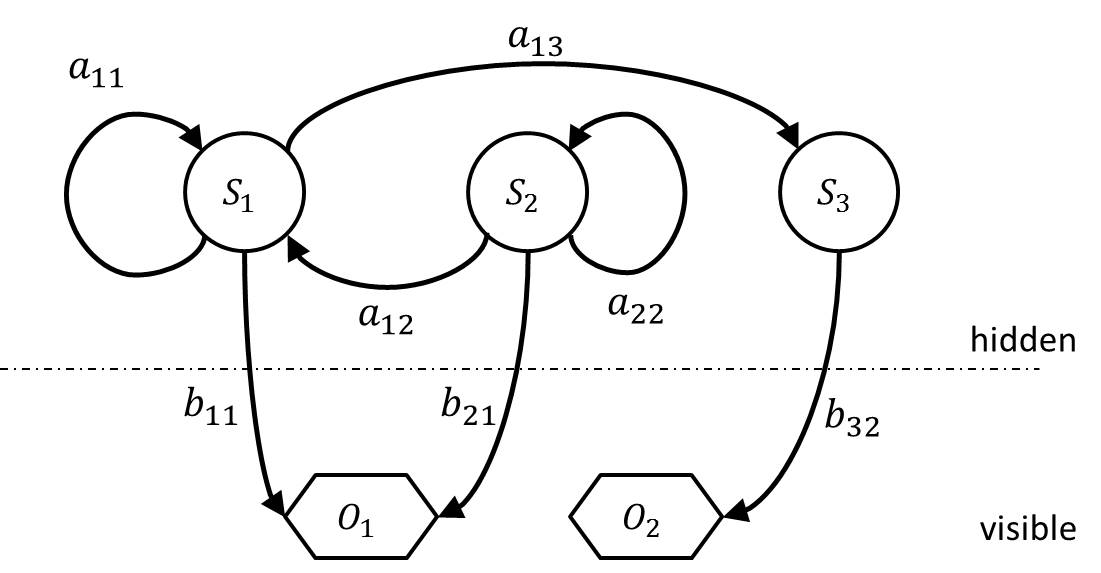
\includegraphics[scale=0.6]{Figures/HMM_simple.jpg}
  \caption[description]{\textbf{HMM Visual representation:} It shows the transition probabilities between three hidden states $\{S_1, S_2, S_3 \}$ and the emission probability transitions $\{b_{11}, b_{21}, b_{32} \}$. Note that the transition probabilities equal to zero are not included, for example: $a_{23}$. Only the observed sequence $O_{t \in [1,T]}$ is observable, the states $\{S_1, S_2, S_3 \}$ that produce the samples are not observable. The emission probability transition $b_{k,t}$ can be any probability function, for example a Gaussian distribution.}
  \label{fig:HHM_MODEL}
\end{figure}

Figure \ref{fig:HHM_MODEL} shows the visual representation of the HMM. It says there is an internal Markov process, that itself cannot be "observed" directly which is called as the "hidden Markov process" (i.e. three hidden states $\{S_1, S_2, S_3 \}$ with their correspondent probability transitions $a_{ij}$). This Markov chain is the responsible for generating observed samples ${O_1, O_2}$ according to the probabilities specified by the matrices $\mathbb{A}$, $\mathbb{B}$ and $\pi$. Once one hidden state is reached, it is said that the state $S_k$ emits an observed sample $O_t$ under the probability $b_{k,t}$. The sequence of hidden states $\mathbb{S}$ that generated the observed sequence $\mathbb{O}$ can be revealed by solving the decoding problem that is explained in section \ref{sec:decoding_HMM}. 




\subsection{Gaussian Hidden Markov Model}

To overcome certain predefined weaknesses of the standard HMM, new ways to combine HMM with other approaches or new models have been proposed (\citeauthor{ghahramani2001introduction}, 2001 \cite{ghahramani2001introduction}). One extension of the HMM model for continuous observation values is the Gaussian Hidden Markov Model (GaHMM). Here we borrow some of its concepts for a better description of this extension \cite{bilmes1998gentle,murphy2002dynamic}. \\

A Hidden Markov Model is a probabilistic model of the joint probability of a collection of random variables $\{ O_1,O_2, ...,O_T \}$ and $\{ S_1,S_2, ...,S_{\mathbf{K}} \}$. Where the $O_t$ variables are either continuous or discrete observations and the $S_k$ variables are hidden and discrete. The term discrete for the hidden states implies that we only have $\mathbf{K}$ possible categorical states. Two assumptions make this model tractable, which are defined in equations \ref{horizon_ass} and \ref{independence_ass}. Furthermore, it is assumed that the underlying 'hidden' Markov chain defined by $P(S_t |S_{t-1})$ is time-homogeneous (i.e. it respects the stationary process assumption, equation \ref{stationary_ass}). The hidden Markov chain is represented by the time-independent stochastic matrix $\mathbb{A}$ and the special case when $t=1$ is described by the initial state distribution $\pi$. Now, if the observations $O_i$ are discrete symbols, we can represent the observation model as the matrix $\mathbb{B}$ where $b_{k,t} = P(O_t|S_k)$, but if the observations $O_i$ are a vector in $\rm I\!R^{L}$, it is common practice to use a continuous probability density function, instead of a set of discrete probabilities. GaHMM represents $b_{k,t}$ using a Gaussian distribution: 

\begin{equation}
P(O_t=y|S_t = x) = \Gamma  (y;\mu_x,E_x) 
\label{g_prob_gua_ec}
\end{equation}

Where $\Gamma  (y;\mu, E) $ is the Gaussian density function with a mean vector $\mu_x$ and the variance covariance matrix $E$ evaluated at $y$:   

\begin{equation}
\Gamma (y;\mu,E) =  \frac{1}{(2\pi)^{L/2} \sqrt{ \parallel E \parallel}} exp \Big[ -\frac{1}{2}(y - \mu)^{\intercal} E^{-1}(y - \mu) \Big]  \quad \quad  \text{\footnotemark} 
\label{density_function_b}
\end{equation} 
\footnotetext{Note that $\intercal$ is the symbol for the vector/matrix transpose and $L$ is the cardinality of $\mu_x$.}


A more flexible representation of the GaHMM model is a mixture of $\mathbf{K}$ Gaussians:

\begin{equation}
P(O_t=y|S_t = x) = \sum_{m=1}^{\mathbf{K}} P(M_t=m|S_t=x) \Gamma(y;\mu_{(m,x)},E_{(m,x)})
\label{mixture_gausssian}
\end{equation}
 
where $M_t$ is a hidden variable that specifies which mixture component to use, and $P(M_t=m|S_t=x) = C(x,m)$ is the conditional prior weight of each mixture component \cite{murphy2002dynamic}. In other words, this is the sum of all mixture components with their correspondent distribution, so that all together it represents the probability of an observed sample $O_t$ occurring at time t when the hidden state is equal to $x$. At the end, each hidden state $S_{i}$ is defined by a mean vector $\mu_x$ with his distribution represented by variance-covariance matrix $E_x$.   


\subsubsection{The three problems to solve using HMM}
\label{sec:problems}

HMM is used to solve three kind of problems that are: the learning, evaluation and decoding problem. The solution of these problems is the core of our proposition. In the modeling process, explained in section \ref{modeling}, one finds the libraries that solve each of them. Basically, our proposition find the best HMM models to discover all the possible patterns into the observed sample $\mathbb{O}$. The theoretical details are explained briefly in this section, and the whole implemented process in section \ref{sec:training_process}. The following explains the general idea of the process:
  
\begin{itemize}
\item Learning/ training process: The HMM model is fitted with the observed samples $\mathbb{O} = (O_1, O_T)$. The definition of the observed samples is very important since it defines the kind of HMM to use.
\item Evaluation process: Here one uses the log probability of $P(\mathbb{O} |\mathbb{S}, \lambda)$ (i.e. equation \ref{independence_ass}), to select the best trained model. The model that fits the best the parameters of $\lambda$ is the one who has the greatest probability.
\item Decoding process: When one obtain the best model, there is a perfect matching between the observed samples $\mathbb{O}$ and the sequences of states $\mathbb{S}$. One says that each hidden state $S_k$ emits one sample $O_i$. This is graphically explained in section \ref{sec:profile_model}. We use this mechanism to cluster similar observed samples.  
\end{itemize}

Here the theoretical details. Using the Markov assumptions (i.e. \ref{horizon_ass}, \ref{independence_ass}, \ref{stationary_ass}), one can answer questions about the observed sequence, the hidden sequence, or the model parameters $\lambda$. These related questions are known as the three basic problems of HMM. This work does not go into detail about these three questions, but the reader is invited to refer to an excellent tutorial in \cite{bilmes1998gentle}, and more related literature of HMM in \cite{haussler1996generalized, ghahramani2001introduction, stamp2004revealing, ramage2007hidden, pfundstein2011hidden}. 


\subparagraph{The Learning Problem}
\label{sec:learning_HMM}

Given an observed sequence $\mathbb{O}$ how can we find the HMM that best fits? HMM has different ways to tune the parameters $\lambda = \{\pi, \mathbb{A}, \mathbb{B} \}$. There are two approaches for the training process, the generative training algorithms and discriminative training algorithms \cite{dymarski2011hidden}. Usually, the solution space of HMMs is coded as a function of $\lambda$ and one can consider two main optimization criteria as being: Maximum Likelihood (ML) and Maximum Mutual Information (MMI). This optimization of parameters $\lambda$ is usually done by gradient algorithms in order to find the maximum likelihood. The Maximum Likelihood Estimation (MLE) can be found by using the Expectation-Maximization algorithm (EM). This algorithm is able to deal with derivatives of the likelihood function with respect to all the unknown values of $\lambda$ by picking arbitrary values for one set of unknown parameters, and then using the previous set, to estimate a second set of parameters, and then apply this procedure recursively until the convergence of parameters. In general, this process generates multiple solutions, so there is no guarantee that the global maximum will be found \cite{dymarski2011hidden}. Our proposed method uses EM algorithm to tune the $\lambda$ parameters, and the best trained model (i.e. the one that get the maximum likelihood) is elected by doing a k-fold cross validation process. This process is explained in \ref{sec:cross}. 


\subparagraph{The Evaluation Problem}
\label{sec:evaluation_HMM}

In general, one of the benefits of HMM is its evaluation property. The question that involves the observed sequence and the parameters of the model is known as the evaluation problem. The question is formulated as follows: What is the probability that the given observations $\mathbb{O} = (O_1,O_2, ...,O_T )$ can be generated by a Hidden Markov Model with parameter $\lambda = \{\pi, \mathbb{A}, \mathbb{B} \}$. In other words: $p(\mathbb{O}|\lambda) = ?$. The solution to this problem is the use of the forward or backward algorithm that finds $p(\mathbb{O}|\lambda)$ in about $K^{2} T$ multiplications \cite{stamp2004revealing}. The solution to this question can be used to evaluate a trained HMM, or it can also suffice just to know whether or not an observed sequence can be generated/emitted by a given HMM, the latter being used in classification problems. In this study, since we are conducting unsupervised fault discovery and are interested in evaluating our trained models and using the best ones, we can perform fault detection.



\subparagraph{The Decoding Problem}
\label{sec:decoding_HMM}

In some cases, one is interested in finding the "most likely" state sequence of the Markov process, given an observed sequence $\mathbb{O} = (O_1,O_2, ...,O_T ) $. Literature defines "most likely" in at least in two ways: 1. "most likely" is defined as the state sequence with the highest probability from among all possible state sequence of length $T$. 2. "most likely" is defined as the state sequence that maximizes the expected number of correct states \cite{stamp2004revealing}. This study is interested in finding the whole state sequence with maximum likelihood. 

Therefore, the problem is defined as: To find an optimal sequence for the underlying hidden Markov model given a HMM with parameter $\lambda = \{\pi, \mathbb{A}, \mathbb{B} \}$ and an observed sequence $\mathbb{O}$. Stated differently, we want to know the "most likely" hidden state sequence that emitted the observed sequence $\mathbb{O}$. To solve this problem the Viterbi algorithm is used. By using Viterbi algorithm, one can find the sub-sequences of an observation sequence O that best matches to a given hidden Markov model. For the present study, this is the way in which the typical daily patterns are discovered and clustered. Finding the most likely hidden state sequence is the way in which we tag days where there is similar pattern across the entire time series.

 
\subsubsection{Advantages and perils of using Hidden Markov Model}

An HMM is a generative, probabilistic model. This model generates distributions by using the available information from the observed sequence. Because of its capacity for detecting sequences, this model is often used for recognition problems that involve sequence recognition such as speech recognition, gesture recognition, information extraction, recognition of Human Genes in DNA and others \cite{ramage2007hidden, seymore1999learning, haussler1996generalized}. \citeauthor{seymore1999learning}, 1999 \cite{seymore1999learning} stated the advantages and perils of HMMs as follow: 

\begin{quote}
"HMM offers the advantages of having strong statistical foundations that are well-suited to natural language domains, handling new data robustly, and being computationally efficient to develop and evaluate due to the existence of established training algorithms. The disadvantages of using HMMs are the need for an a priori notion of the model topology and, as with anystatistical technique, large amounts of training data".
\end{quote}

Later, \citeauthor{ghahramani2001introduction}, 2001 \cite{ghahramani2001introduction} showed that HMMs are a kind of Bayesian Network because it is possible to derive the HMM algorithms from more general algorithms for Bayesian networks. He also explained how to overcome some weakness of HMM models (due to the unconstrained transition matrix $\mathbb{A}$ and the exponential number of states in the model) by creating more general models for HMM such as factorial HMMs and tree-structured HMMs. \\ 


\subsection{Hierarchical clustering}
\label{hierarchical}

Hierarchical clustering seeks to build a hierarchical structure of observed objects in a recursive fashion. Two methods are identified: \textbf{1. Agglomerative.}  This is a "bottom up" approach, each object starts in its own cluster. Then clusters are successively merged until the desired cluster structure is obtained. \textbf{2. Divisive} This is a "top down" approach, all objects belong to one cluster. Then the cluster is divided into sub-clusters, which are successively divided into their own sub-clusters. This process continues until to reach the desired structure \cite{maimon2007soft}. Since the \textit{GaHMM profile} model described in section \ref{sec:profile_model} discovers the existing daily patterns into the time series of the variables, we need an strategy to group cluster profiles in a "bottom up" fashion, creating in this way groups of cluster profiles. There are abundant literature about similarity distances and linkage methods  \footnote{Rules that serve as criteria for joining similar objects} for hierarchical clustering, the reader is invited to see more details about the set of metrics and linkage methods in \cite{saraccli2013comparison,mullner2011modern,maimon2007soft}. We describe in section \ref{sec:hierar_agg}, the use of the hierarchical agglomerative clustering for grouping the discovered cluster profiles.

 

\subsection{Symbolic Aggregate Approximation (SAX) transformation}
\label{section:SAX}

SAX allows the representation of time-series data in words of a finite alphabet $A$. This approach was developed by \citeauthor{keogh2005hot}, 2007 \cite{lin2007experiencing,butler2015sax,keogh2005hot}. The SAX transformation follows this process: The normalized timeseries, Z(t) \footnote{z-scored normalization is applied}, is first broken down into N individual non-overlapping subsequences. This step is known as chunking, and the period length N  is based on a context logical specific period \footnote{Since the interest of this work is to find daily pattern, therefore $N=24$} \cite{lin2007experiencing}. In the next step, each sunsequence of the time series is divided into W equal sized segments. The mean of the points in each small segments is calculated and an alphabetic character from $A$ is assigned according to the table in \ref{table_sax} \cite{lin2007experiencing}. To do this asignation, each mean values that falls in zones between the vertical breakpoints, $B= \beta_1,..., \beta_a - 1$ is substituted by a symbol. Figure \ref{SAX_transf} \cite{lin2007experiencing} exemplify the concept, where the time series (blue line) is transformed into the correspondent word "baabccbc". This approach is used in DayFilter approach \cite{miller2015automated}, which is considered as one of the way to detect daily profiles in the state of the art \cite{kim2017review}. The SAX method can convert time series data with an equivalent symbolic representation for identifying relevant patterns by comparing strings. \citeauthor{miller2015automated}, 2015 \cite{miller2015automated} presented how the SAX method can be implemented to detect the schedules using total building power measurement. \citeauthor{miller2015automated} performed pattern discovery over two different power measurement time series data of the energy consumption of two buildings. His analysis imply among other issues, the identification of discord profiles that implied high corruption of energy \cite{kim2017review, miller2015automated}. The SAX approach is compared against our proposed \textit{GaHMM profile} model in section \ref{comparison_sax_hmm}.


\begin{figure}[h!]
  \vspace{0.5em} %better style
  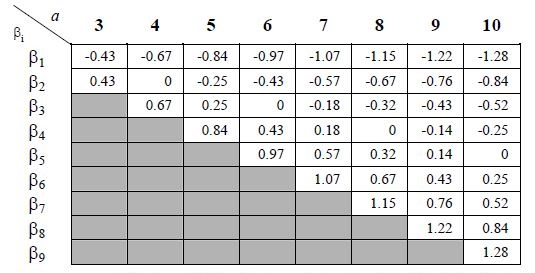
\includegraphics[scale=0.7]{Figures/table_sax.jpg}
  \caption[description]{A lookup table that contains the breakpoints that
divide a Gaussian distribution in an arbitrary number (from 3
to 10) of equiprobable regions}
  \label{table_sax}
\end{figure}

\begin{figure}[h!]
  \vspace{0.5em} %better style
  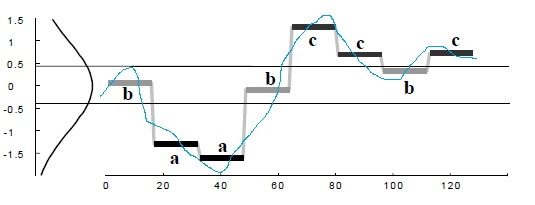
\includegraphics[scale=0.7]{Figures/SAX_transf.jpg}
  \caption{A time series is discretized by first obtaining a PAA approximation and then using predetermined breakpoints to map the PAA coefficients into SAX symbols. In the example above, with n = 128, w = 8 and $A = \{ a, b, c\}$, the time series is mapped to the word baabccbc }
  \label{SAX_transf}
\end{figure} 
 

\section{Data Visualization}

This master thesis does not develop a new data visualization artifact for presenting the discovered information within the multivariate dataset. Developing a new visualization goes beyond our objectives. However, our work uses visualization principles and tools in order to communicate to the reader complex structures of patterns, the interaction between variables, the evaluation of models and the respective results of each section. This task is not a easy task to do since one has to look for visualization that fits the best with the data. In fact, the use of principles, concepts, techniques and theories for data visualization come from multiple backgrounds: programming, web design, semiotic or psychology (\citeauthor{aparicio2014}, 2014 \cite{aparicio2014}). Therefore, choosing one visualization could become a complex situation because it could imply several criteria from different disciplines. In this work, the combination of data mining, and data visualization can be considered as art and science \cite{aparicio2014, kohavi2001data} because there is not strict rules to define which visualization is the most appropriate, and the trial-and-error process is one of the common approaches to use in this domain \cite{kohavi2001data}. Propositions such as Exploratory data analysis (EDA) aims to looking at data for finding descriptive patterns, trends or any hint that help to generate hypothesis of interest of the researcher. However, if this process is made by hand in a high dimensional dataset, it becomes impractical in some cases because of the filtering process \cite{witten2016data}. We believe that the use of data mining techniques in combination with the appropriated visualizations are a powerful tool for knowledge discovery. The reader will see the use of existing visualization artifacts for different purposes. For example, box plots \cite{williamson1989box} are used for a visual evaluation of the cluster quality of cluster profiles in section \ref{sec:eval_all}. Other concept such as the calendar visualizations \cite{van1999cluster} are needed in order to see the distribution of clusters in section \ref{sec:seasonal_model}, and others uses. We expect by the use of data visualizations be able to discover the behavior of the building and represent it in the best possible way. 

\subsection{Hierarchical Edge Bundles}
\label{sec:edge}


Hierarchical Edge Bundles visualization was proposed by \citeauthor{holten2006hierarchical}'s work (2006, \cite{holten2006hierarchical}). This visualization is a compound graph that is based on visually bundling the adjacency edges, i.e., non-hierarchical edges, together. In this way, two or more nodes are joined by using polylines that are bended using a B-spline curve for more readability. This tree visualization based technique can be used in conjunction with other visualizations to express different concepts. Figure \ref{fig:edge} shows an example where this visualization displays adjacency relations between nodes. Colors in the linkage line provide more information about the connection between nodes. 



\begin{figure}[h!]
  \vspace{0.5em} %better style
  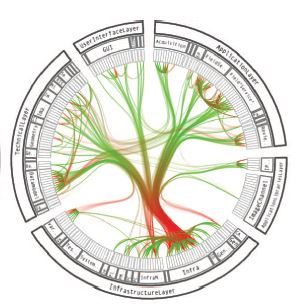
\includegraphics[scale=0.7]{Figures/edge.jpg}
  \caption[description]{Radial layout construction of hierarchical edge bundles}
  \label{fig:edge}
\end{figure}


In our case, we use this visualization to represent the connection between the variables (time series of the measurements) in the building, this can be appreciated as an information visualization who explains the existing linear correlation between variables (i.e. nodes). This visualization was used for the interactional model where each node is a variable of the building dataset and each linkage line represent the linear correlation between them, refer section \ref{sec:interactional_model} for more details. Other variations and more layouts of this visualization are explained in \cite{holten2006hierarchical}. \footnote{Library available on \url{https://bl.ocks.org/mbostock/7607999}}

  